\documentclass[12pt]{article}
\usepackage[utf8]{inputenc}
%\usepackage[margin=1in]{geometry}
\usepackage{amssymb}
\usepackage{amsmath}
\usepackage{mathtools}
\usepackage{amsthm}
\usepackage{setspace}
\usepackage{cancel}
\usepackage{bbm}
\usepackage{pgfplots}
\usepackage{listings}
\usepackage{float}

\usetikzlibrary{arrows, calc, patterns, shapes}
  \pgfplotsset{compat=1.15}
\renewcommand{\baselinestretch}{1.25}
\newcommand\sbullet[1][.5]{\mathbin{\vcenter{\hbox{\scalebox{#1}{$\bullet$}}}}}
\newcommand{\indep}{\perp \hspace{-.5 em} \perp}
\def\E{\mathbb{E}}
\def\e{\mathcal{E}}
\def\d{\mathcal{D}}
\def\I{I_n}
\def\l{\ell}
\def\sumn{\sum^n_{i=1}}
\def\i{\mathcal{J}}
\def\x{\mathbf{X}}
\def\inv{^{-1}}
\def\f{Fréchet }
\newcommand{\til}[1]{\underset{\sim}{#1}}
\newcommand\expp[1]{\exp\bigg\{#1\bigg\}}
\newcommand\der[2]{\frac{\partial #1}{\partial #2}}
\newcommand{\ds}{\displaystyle}
\lstset{frame=tb,
  language=Python,
  aboveskip=3mm,
  belowskip=3mm,
  showstringspaces=false,
  columns=flexible,
  basicstyle={\small\ttfamily},
  numbers=none,
  numberstyle=\tiny\color{gray},
  keywordstyle=\color{blue},
  commentstyle=\color{red},
  stringstyle=\color{mauve},
  breaklines=true,
  breakatwhitespace=true,
  tabsize=3
}
\theoremstyle{definition}
\newtheorem{theorem}{Theorem}

\theoremstyle{definition}
\newtheorem{definition}{Definition}

\newtheorem{example}{Example}[section]

\let\inf\infty
\title{Math 80622A Final Report}
\author{Jean-Yves Djamen }
\date{Fall 2020}

\begin{document}

\maketitle
\tableofcontents{}
\doublespacing

\pagebreak


\section{Preface}
Statistical extreme value theory is a popular toolbox used in the modeling of infrequent (or extreme) events. It has been shown to be effective at several tasks, from the analysis of weather patterns \cite{test1} to financial stocks \cite{test2}. One tool in this toolbox is the generalized Pareto distribution which is used to model exceedences of data over a set threshold. While this tool is popular, there are practical difficulties that may arise when trying to find an appropriate threshold over which to fit data. In their work, \cite{papatawn} Jonathan Tawn and Ioannis Papastathopoulos propose a new class of models to extend the generalized Pareto distribution and mitigate the practical difficulties encountered from its use. In this report, reproduction of their analyses will be conducted alongside new analysis using their model extensions on new data. 

\section{Generalized Pareto Model}
Given a random variables, $X$, with cdf $F_X$ and $u_F$ defined as $u_F= \sup\{x: F_X(x)<1\}$ there is  a limiting result \cite{gpd} for the conditional distribution $X-u|X>u$ 
\[ \lim_{u\rightarrow u_F }P(X-u < y|X>u) = 1-\bigg( 1+ \frac{\xi y}{\sigma}\bigg)^{-1/\xi} \tag{1}\]
Where (1) is the cumulative distribution function (cdf) of a generalized Pareto (GP) distribution with parameters $\sigma$ as the scale and $\xi$ as the tail index. Once this result holds for a threshold $u<u_F$, it will hold for all thresholds $u'>u$. As previously mentioned, finding an appropriate threshold $u$ to use in practice can be a challenging problem. Standard methods include fitting GP models over a range of thresholds, then plotting the modified scale ($\sigma^*$) defined below over a varying range of thresholds. The minimum threshold after which $\sigma^*$ stabilizes is then chosen as the threshold.
\[\sigma^*= \sigma_u-\xi u\]
In practice, such a threshold may not exist or may be too large relative to the data at hand. Large thresholds result in loss of data and high variance in the estimated parameters. For this reason, \cite{papatawn} proposes 3 new models to serve as extensions to the GP distribution. 

\section{Extended Generalized Pareto Models}
Let $U\sim \mathcal{U}(0,1)$ be a uniform random variable defined on (0,1) and let $G$ be the cdf of a GP$(\sigma,\xi)$. Then, by standard statistical calculations (probability integral transform) the new random variable defined as $V=G^{-1}(U)$ also follows a GP distribution. To form their extended models, \cite{papatawn} use a similar logic. This extension mechanism makes use of a pseudo probability integral transform $V=G^{-1}(Y)$ where $G$ is as before and $Y$ is a single parameter random variable with support on the unit interval. With the appropriate choice of distribution $Y$, the random variable $V$ will follow distribution EGP$(\kappa, \sigma,\xi)$ where $\xi$ is conserved as the tail index \cite{papatawn}. Furthermore, for a specific value $\kappa^*$, EGP$(\kappa^*, \sigma,\xi)$=GP$(\sigma,\xi)$ thus connecting the base distribution to the proposed extensions. 

\subsection{Extended Distributions}
As this report is not meant to reproduce $\cite{papatawn}$, this section serves only as a place to define the proposed models for later reference. First, the probability density function of the three models  arising from the extension mechanism discussed above. \footnote{Be denotes the beta function}
\begin{align*}
g_{EGP1}(x,\kappa,\sigma,\xi)&=\begin{cases} \frac{|\xi|/\sigma}{\text{Be}(\kappa, |\xi|^{-1})}\{1-(1+\xi x/\sigma)_+^{-|\xi|/\xi}\}^{\kappa-1} (1+\xi x/\sigma)_+^{-1/\xi-1} & \xi \neq 0\\\\
    \frac{\sigma^{-1}}{\Gamma(\kappa)}x^{\kappa-1}e^{-x/\sigma} & \xi \rightarrow 0
    \end{cases}\\
g_{EGP2}(x,\kappa,\sigma,\xi)&= \begin{cases}\frac{\sigma^{-1}}{\Gamma(\kappa)}\{\xi^{-1}\log(1+\xi x/\sigma)_+\}^{\kappa-1} (1+\xi x/\sigma)_+^{-1/\xi-1} & \xi\neq 0\\\\
    \frac{\sigma^{-1}}{\Gamma(\kappa)}x^{\kappa-1}e^{-x/\sigma} & \xi\rightarrow 0
    \end{cases}\\
    g_{EGP3}(x,\kappa,\sigma,\xi)&= \begin{cases} \frac{\kappa}{\sigma}\{1-(1+\xi x/\sigma)^{\kappa-1}(1+\xi x/\sigma)_+^{-1/\xi-1}\} & \xi \neq 0\\\\
    \frac{\kappa}{\sigma}(1-e^{-x/\sigma})^{\kappa-1}e^{-x/\sigma} & \xi \rightarrow 0
    \end{cases}
\end{align*}
Next, the corresponding likelihood functions used to estimate parameters from the fit of these models to data. Given a random sample $\boldsymbol x$ of $n_u$ exceedences over $u$, the corresponding model likelihoods are given as follows:
\begin{align*}
    \ell^{EGP1}(\kappa, \sigma,\xi|\boldsymbol{x})=&n_u\log\bigg\{ \frac{|\xi|/\sigma} {Be(\kappa, |\xi|^{-1}}\bigg\}+(\kappa-1)\sum_{i=1}^{n_u}\log[1-\{1+\xi(x_i-u)/\sigma\}_+^{-|\xi|/\xi}]\\
    &-(1/\xi+1)\sum_{i=1}^{n_u}\log\{1+\xi(x_i-u)/\sigma\}_+\\
    \ell^{EGP2}(\kappa, \sigma,\xi|\boldsymbol{x})=&n_u\log\bigg\{ \frac{\sigma^{-1}}{\Gamma(\kappa)}\bigg\}+(\kappa-1)\sum_{i=1}^{n_u}\log[\xi^{-1}\log\{1_\xi(x_i-u)/\sigma\}_+]\\
    &-(1/\xi+1)\sum_{i=1}^{n_u}\log\{1+\xi(x_i-u)/\sigma\}_+\\
    \ell^{EGP3}(\kappa, \sigma,\xi|\boldsymbol{x})=&n_u\log(\kappa/\sigma)+(\kappa-1)\sum_{i=1}^{n_u}\log[1-\{1+\xi(x_i-u)/\sigma\}_+^{-1/\xi}]\\
    &-(1/\xi+1)\sum_{i=1}^{n_u}\log\{1+\xi(x_i-u)/\sigma\}_+
\end{align*}
Finally, given the probability of an exceedance $\zeta_u$, the $T$-observation return levels can be computed. \footnote{$\gamma^{-1}, \beta^{-1}$ are the inverses of the incomplete gamma and beta functions respectively}
\begin{align*}
    x_T^{EGP1}&= u + \frac{\sigma}{\xi} [\{1-\beta^{-1}(1-(T\zeta_u)^{-1},\kappa, |\xi|^{-1})\}{\-\xi/|\xi|}-1]\\
    x_T^{EGP2}&= u + \frac{\sigma}{\xi} [\exp\{\xi\gamma^{-1}(\kappa,1-(T\zeta_u)^{-1})\}-1]\\
    x_T^{EGP3}&= u + \frac{\sigma}{\xi}[\{1-(1-(T\zeta_u)^{-1/\kappa})\}^{-\xi}-1]
\end{align*}

\subsection{Extension to Available Tools }
In the proposal of these extended generalized Pareto (EGP) models, \cite{papatawn} gives plenty of motivation for the use of EGPs in conjunction to the standard GP. First, the increased flexibility of EGPs induced by parameter $\kappa$ may allow the fitting of EGPs over a lower threshold than can be fitted over a GP. This could yield models with more reliability and statistical power as they utilize more data. Additionally, since EGP(1,$\sigma,\xi$)=GP$(\sigma,\xi$), the EGPs can produce more diagnostics for the GP distribution \cite{papatawn}. Plotting the estimated parameters from an EGP fit along varying thresholds and selecting the minimum threshold after which $\kappa$ is not significantly different from 1 (using confidence intervals), the modified scale and tail index are constant could be used as a heuristic test to assess the validity of the GP model. Though not excessively discussed in \cite{papatawn} this method could provide a correspondence between EGPs and GP models. This correspondence is explored in both the reproduced and novel set of experiments.


\section{Simulation Study}
In the simulation study from \cite{papatawn}, 10000 samples of size $n=100,1000, 10000$ data points generated from a distribution $\mathcal{D}$. For $\mathcal{D}$, the distributions used are Normal(0,1), Student's $t_2$, and Beta(1.5,3) motivated by \cite{papatawn} as representing three domains of attraction $\xi<0, \xi=0, \xi>0$ respectively. The first criticism of \cite{papatawn} comes from its formulation of this simulation. The tail index assignment is false as calculations from \cite{index} indicate. Nevertheless, for each sample, an EGP1, EGP2 and GP model is fit over a range of equally spaced thresholds. The root mean square error for estimating the $T_1, T_2$ \footnote{$T_1=n*1.5 , T_2=n*5$} observation return level is compared across models. In the reproduction of this experiment, the sample size is reduced from 10000 to 250. 

Due to this reduced number of samples, some observations in \cite{papatawn} were unable to be reproduced. Primarily amongst these is the observation that the distance between the optimal threshold (where minimum RMSE occurs) for the EGP1 and GP gets smaller as $n$ grows. Table 1 depicts the optimal thresholds for estimation of return levels of each sample size. From this table, it is apparent that the distance between the RMSE from the EGP1 and GP model from the reproduction experiment does not decrease as size increase.

\begin{table}[H]
    \centering
    \begin{tabular}{||c|c|c|c||}\hline
\multicolumn{4}{||c||}{$T_1$}\\\hline\hline
    Model& $n=100$& $n=1000$& $n=10000$\\\hline
    $u_{EGP}$ & -2.5(-2.32)& -0.23 (0.05) & 0.09(1.48)  \\
     $u_{GP}$& -2.5 (-0.33) & -2.5 (0.45) & -0.067(1.70)\\\hline\hline
     \multicolumn{4}{||c||}{$T_2$}\\\hline\hline
     $u_{EGP}$ & -2.5(-2.32)& -0.163 (0.51) & 0.492(1.44)  \\
     $u_{GP}$& -2.5 (-0.23) & -0.0049 (0.68) & 0.305(1.44)\\\hline
\end{tabular}
    \caption{Optimal Threshold for estimation of long and short term return levels for each sample size. In parenthesis are the original values from \cite{papatawn}. }
\end{table}

A comparison of Figure 1 (original experiment) and Figure 2 (reproduction) shows some consistency of results across studies. The consistent conclusion being, with smaller data size $(n=100)$ the EGPs perform better than the GP models. In fact, with $n=100$, the EGP1 model performs best when fit to on exceedences over the smallest possible threshold thus highlighting the advantage of fitting EGPs (rather than GPs) when working with smaller datasets.

\begin{figure}[H]
\begin{center}
{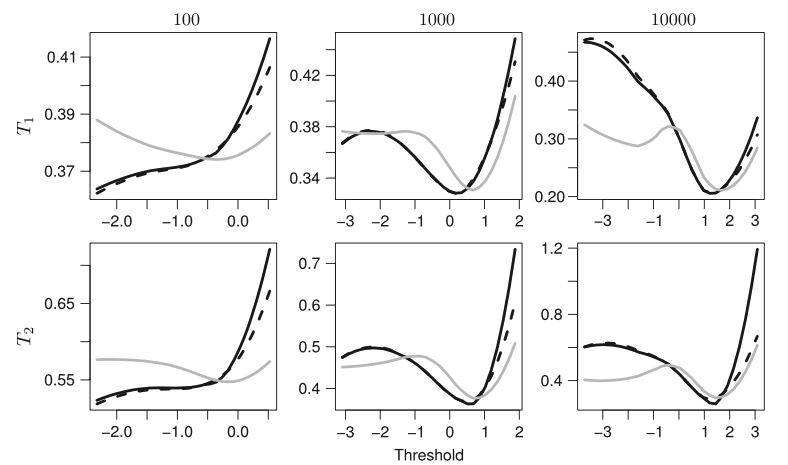
\includegraphics[width=4.0in]{project/papafiles/fig2.papa.png}}
\caption{RMSE for the $T_1$(top row) and $T_2$(bottom row) return level estimates from EGP1(black), EGP2(dashed) and GP (gray) from experiment in \cite{papatawn} with standard normal data.}
\end{center}
\end{figure}
\begin{figure}[H]
\begin{center}
{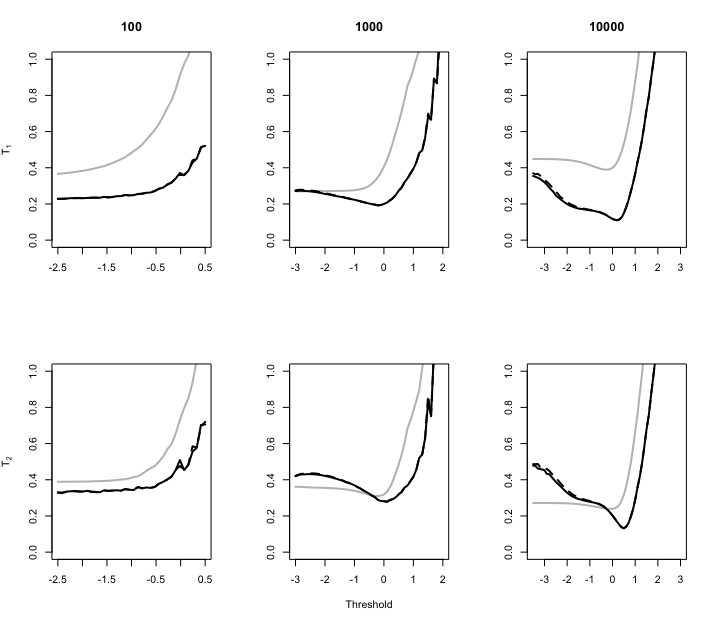
\includegraphics[width=4.0in]{project/papafiles/fig2.me.png}}
\caption{RMSE for the $T_1$(top row) and $T_2$(bottom row) return level estimates from EGP1(black), EGP2(dashed) and GP (gray) from experiment reproduction.}
\end{center}
\end{figure}
Recall that one of the proposed applications of EGP models was as a diagnostic tool for GPs through observation of estimated $\kappa$ values plotted against varying thresholds. In Figure 3, this diagnostic tool is depicted. Similarly to the analysis in \cite{papatawn} the reproduced experiments show that the threshold for which the value 1 is inside the confidence interval for $\kappa$ corresponds (approximately) to the threshold that yields the minimum RMSE with the GP model. It should be noted that this is slightly less accurate for small samples sizes ($n=100$) in both the original and reproduction experiments.

\begin{figure}[H]
\begin{center}
{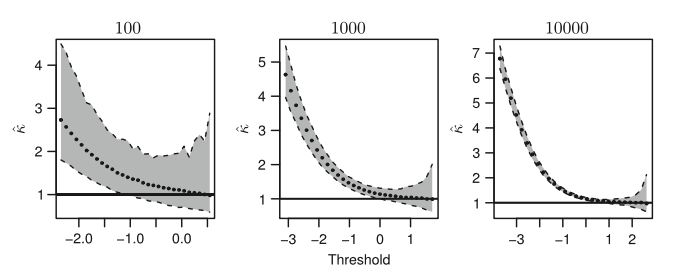
\includegraphics[width=4.0in]{project/papafiles/fig3.papa.png}}
{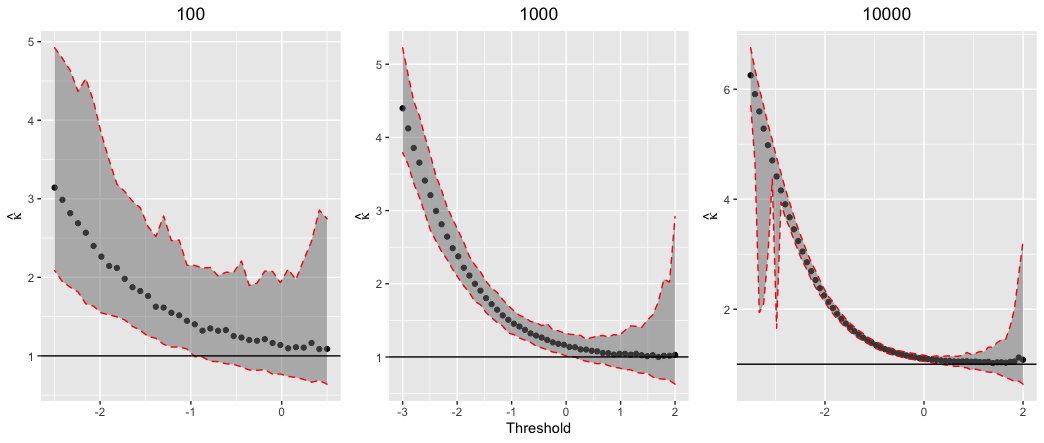
\includegraphics[width=4.0in]{project/papafiles/fig3.me.png}}
\caption{Median Monte Carlo estimates of $\kappa$ parameter plotted against each threshold for each sample size along with the 95\% Monte Carlo confidence intervals (grey). Original experiment from \cite{papatawn}(top) and reproduced experiment (bottom). }
\end{center}
\end{figure}

\begin{figure}[H]
\begin{center}
{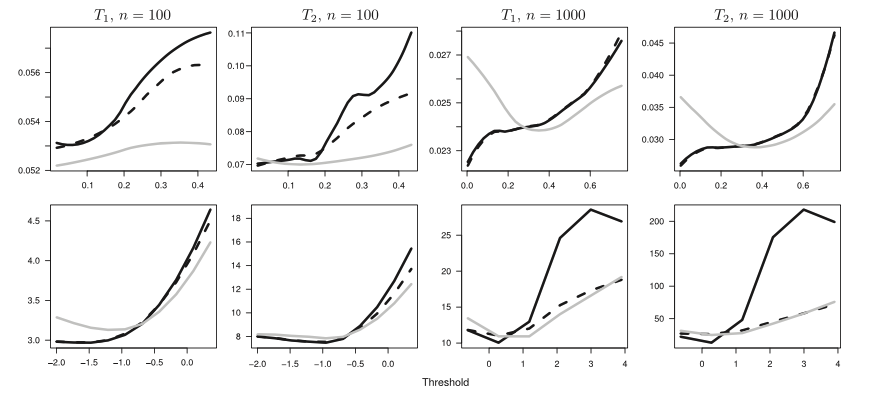
\includegraphics[width=4.0in]{project/papafiles/fig4.papa.png}}
\caption{RMSE for the $T_1$(top row) and $T_2$(bottom row) return level estimates from EGP1(black), EGP2(dashed) and GP (gray) from \cite{papatawn} simulation. First row corresponds to Beta(1.5,3) and the second to Student's $t_2$ data.}
\end{center}
\end{figure}
\begin{figure}[H]
\begin{center}
{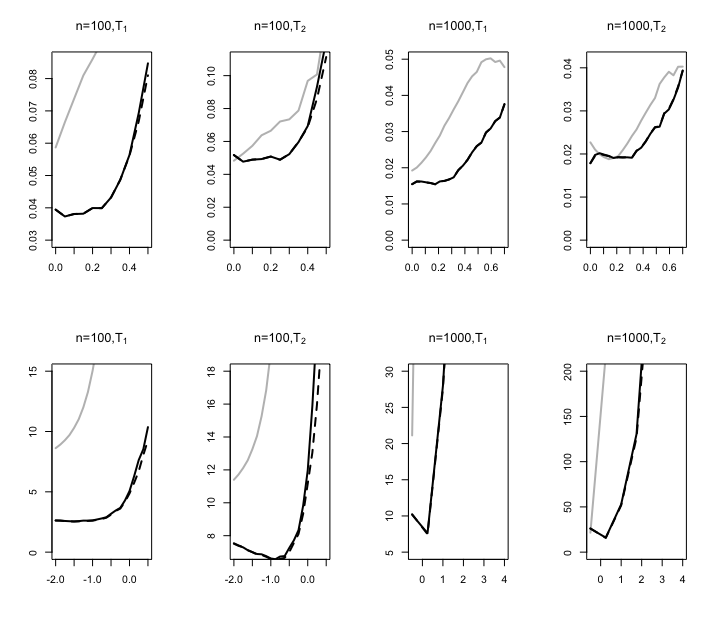
\includegraphics[width=4.0in]{project/papafiles/fig4.me.png}}
\caption{RMSE for the $T_1$(top row) and $T_2$(bottom row) return level estimates from EGP1(black), EGP2(dashed) and GP (gray) from reproduced simulation. First row corresponds to Beta(1.5,3) and the second to Student's $t_2$ data.}
\end{center}
\end{figure}

While the discussion so far has been focused on the simulation with standard normal data, Fig. 4 and Fig. 5 show the RMSE output of the simulation studies (original and reproduction respectively) with the other distributions. From these, the conclusions are the same: the EGP models perform better than the GP for T-observation return level inference.

\section{Application to River Nidd Data}
This experiment uses the 154 exceedences over the threshold 65.08 $m^3/s$ of the flow of the river Nidd gathered from 1934 to 1969. In this analysis, \cite{papatawn} fits an EGP1 and a GP over a range of threshold (of length 40) varying from 65.08 to 88.61. The purpose of this analysis is three fold. First, to display the ability of the EGP1 model to perform competitively against the GP while using a lower threshold. Then, to underline the diagnostic ability of EGP1 for GP models through threshold selection. Finally, to illustrate the return level stability unique to the EGP. Though this experiment was not perfectly reproduced, sections 5.1-5.3 discuss its intent and addresses the reproducibility issues. 

\subsection{Selection Lower Thresholds}
First, \cite{papatawn} aim to demonstrate that the extensions to the GP can be fitted over smaller thresholds (and thus include more data). The graph below contains the parameter estimates for both the EGP1 and GP models as calculated by \cite{papatawn}. From this, the threshold $u=65.08$ is chosen for the EGP1 model.
\begin{figure}[H]
\begin{center}
{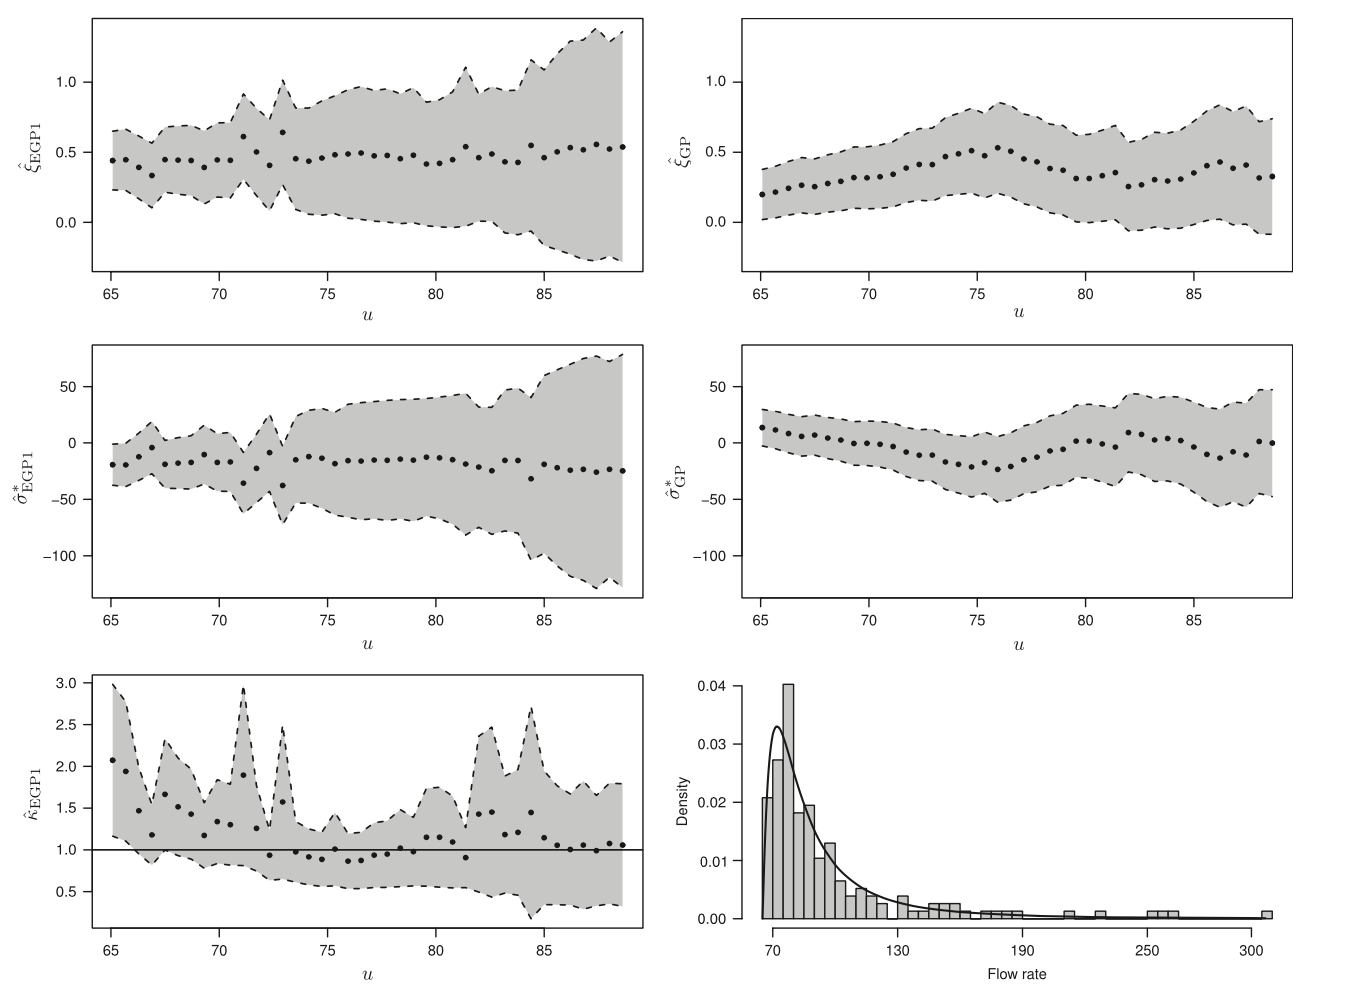
\includegraphics[width=5.0in]{project/papafiles/fig5 papa.png}}
\caption{Figure 5 from \cite{papatawn} of maximum likelihood estimates from 95\% confidence intervals from fitting EGP1 (left column) and GP (right column). The bottom right graph shows histogram of river Nidd data over layed with EGP1 fitted model with $u=65.08$ }
\end{center}
\end{figure}
Following this analysis, \cite{papatawn} observe that the minimum value $u$ for which $\hat\kappa$ is not significantly different from 0 is $75.3$ and remark that this choice of threshold consistent with the threshold resulting from a different analysis \cite{fig5} and thus use $u=75.3$ for the GP. A criticism from this analysis as performed by \cite{papatawn} is the lack of diagnostic plot from either fit. While the EGP1 may seem to have stable estimated parameters over varying thresholds, a quantile-quantile(qq) plot or probability-probability(pp) plot would give more information about the statistical power of the EGP1 model in comparison to the GP.
%TODO INSERT QQ PLOTS

Below are the graphs resulting in the reproduction of the Nidd data analysis. While the graph of the $\hat\kappa$ parameter over varying $u$ is similar to the one in the original experiment, this report has failed to exactly reproduce the figures from the previous graph.


%\subsection{EGP1 for GP Threshold Selection}
%Next, by plotting the samples estimates (and corresponding confidence intervals) for $\hat\kappa$, \cite{papatawn} aims to show the use of EGP1 in choosing a threshold for a GP.

\subsection{EGP1 Return Level Stability}
Finally, \cite{papatawn} displays the stability of return level estimates from an EGP1 model by comparing them to those of an EGP2 model. Below are the stability plots for the EGP1 and GP model from the original analysis and an attempt at reproduction. 
%todo Return level estimates go here 

Again, attempting the reproduction of the graphs is imperfect. In fact, from the reproduction analysis, it appears that the GP estimates are more stable than the EGP estimates. This agrees with the reproduction graphs show in figure 6 as the GP parameter estimates seem more stable than those of the EGP1. Also, there is the same criticism to this analysis as the previous one since return level stability and accuracy are not the same. By omiting 

\section{Application to Pharmaceutical Data}


\section{Application to Precipitation data - Rain}


\section{Application to Precipitation data - Snow}


\section{Conclusions}

 
\cite{papatawn}

\bibliographystyle{plain}
\bibliography{refs}
\end{document}